\subsection{PsykologNords problemstilling}
\label{section:problemstilling}

PsykologNord bruger to informationssystemer til at understøtte deres forretning, se figur \ref{forretning:isfml}.
Dinero bruges som deres regnskabsprogram til at lave og sende fakturaer til deres klienter.

TerapeutBooking er deres nuværende bookingsystem.
Som det kan ses på figur 3 understøttes virksomheden meget af de to informationssystemer, og derfor er det vigtigt for dem, at de fungerer godt.

PsykologNord har følgende problemer med TerapeutBooking:

\begin{itemize}
    \item TerapeutBooking kan ikke håndtere en bruger tilknyttet flere lokationer.
    Derfor har Katrine to forskellige kalendere: En for hendes klienter i Aarhus og en i Aalborg.
    Det har den konsekvens, at Katrine eller Jean manuelt skal blokere hendes ene kalender, når hun booker en tid i den anden kalender med en klient.
    
    \item TerapeutBooking kan ikke håndtere flere kalendere, der bruger de samme lokaler.
    Det betyder, at da Miriam og Katrine lige nu begge tilbyder samtaleterapi i Aarhus og Aalborg, skal de manuelt gå ind og blokere aftaler i hinandens kalendere.
    Hvis Katrine har en aftale i Aalborg om mandagen klokken 10 til 11, skal hun eller deres sekretær blokere tiden i Miriams kalender
    
   \item PsykologNord har som beskrevet i afsnit \ref{section:forretningsmodel} flere psykologer tilknyttet deres firma.
   Men TerapeutBooking giver ikke en tilfredsstillende måde at styre deres brugeres rettigheder på.
   En bruger kan få lov til at ændre alle journaler, se alle journaler eller se ingen journaler.
   Det samme gælder for fakturaer.
\end{itemize}

De første to problemstillinger betyder, at noget så simpelt som at lave en aftale med en klient går hen og bliver en tidskrævende proces, hvor der også nemt kan ske fejl, se figur \ref{bilag:bpmnnow} i bilagene på side \pageref{bilag:bpmnnow} for en BPMN over den nuværende process.
Ifølge Katrine bruger Jean lige nu tre timer om ugen på bare at håndtere det merarbejde, de første to problemstillinger forårsager.
Den tredje problemstilling gør, at de ikke kan udvide mere, uden at det kommer til at drukne i et bureaukratisk mareridt ifølge dem selv.

Under vores møder med PsykologNord har de givet udtryk for ønsker om at udvide og bruge lokalerne til et nyt start-up projekt, når de ikke bliver brugt af PsykologNord.
Derfor er det et problem, at deres kalendersystem ikke kan håndtere, at firmaet har flere lokaler.

Det vil blive et stort sikkerhedsproblem, hvis flere forskellige firmaer har direkte adgang til hinandens kunder og deres fortrolige oplysninger.


\begin{figure}[H]
    \caption{Informationssystemers understøttelse af FML}
    \centering
        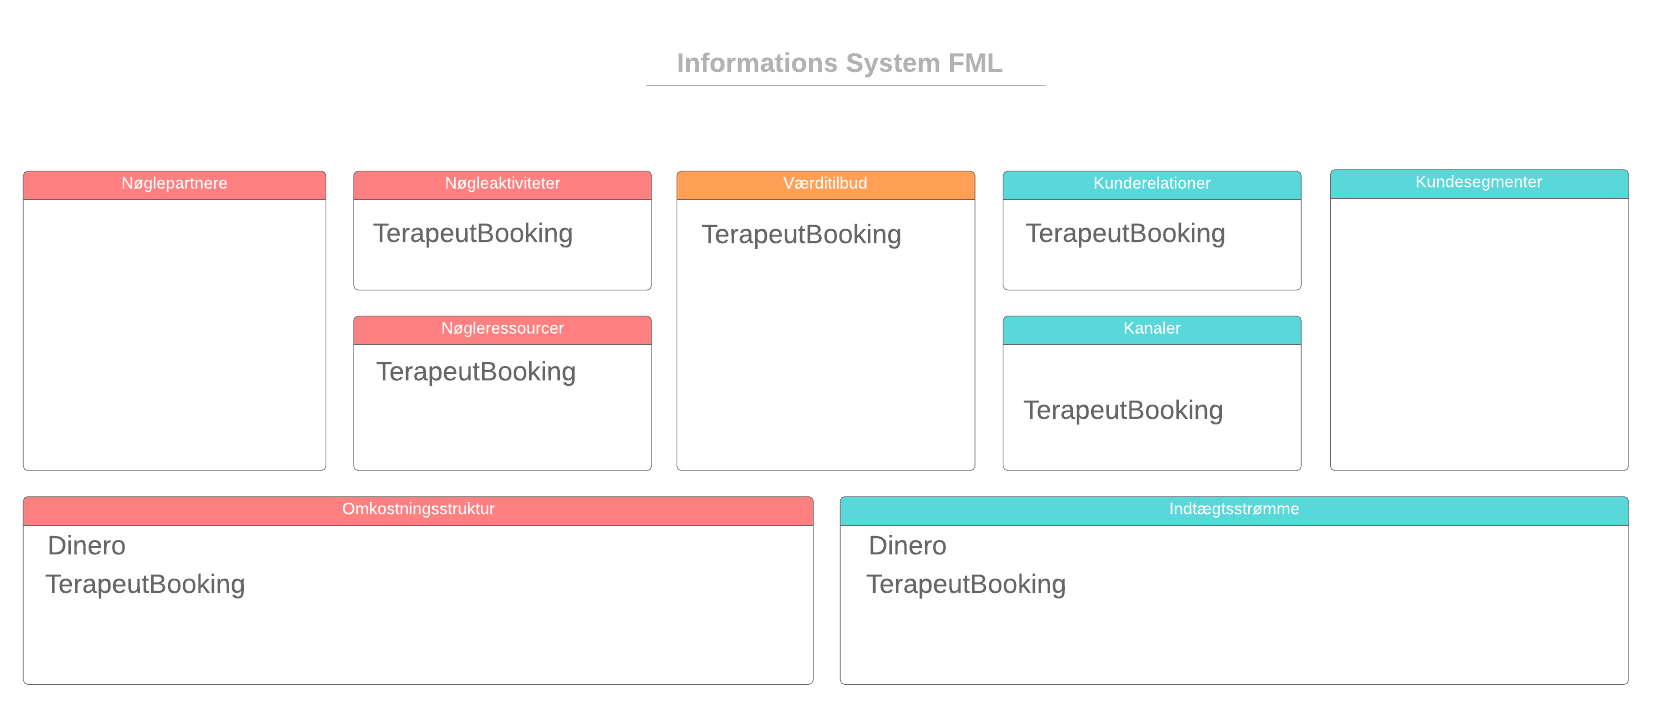
\includegraphics[width=\textwidth]{ISFML.png}
    \label{forretning:isfml}
\end{figure}


